\documentclass[a4paper,11pt]{article}
\input{/home/tof/Documents/Cozy/latex-include/preambule_lua.tex}
\newcommand{\showprof}{show them}  % comment this line if you don't want to see todo environment
\fancyhead[L]{Exercices arbre binaire}
\newdate{madate}{10}{09}{2020}
%\fancyhead[R]{\displaydate{madate}} %\today
%\fancyhead[R]{Seconde - SNT}
%\fancyhead[R]{Première - NSI}
\fancyhead[R]{Terminale - NSI}
\fancyfoot[L]{~\\Christophe Viroulaud}
\AtEndDocument{\label{lastpage}}
\fancyfoot[C]{\textbf{Page \thepage/\pageref{lastpage}}}
\fancyfoot[R]{\includegraphics[width=2cm,align=t]{/home/tof/Documents/Cozy/latex-include/cc.png}}
\usepackage{tikz}

\begin{document}
\begin{Form}
\begin{commentprof}
exercices-arbre-binaire.zip sur site
\end{commentprof}
\begin{center}
\shadowbox{\parbox{16cm}{\centering Télécharger exercices-arbre-binaire.zip sur le site \url{https://cviroulaud.github.io}}}
\end{center}
\begin{exo}
L'arbre figure \ref{arbre} représente une opération arithmétique.
\begin{center}
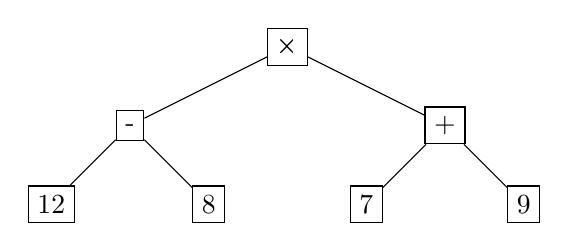
\begin{tikzpicture}
\node[draw] (1) at (0,0) {×};
\node[draw] (2) at (-2,-1) {-};
\node[draw] (3) at (2,-1) {+};
\node[draw] (4) at (-3,-2) {12};
\node[draw] (5) at (-1,-2) {8};
\node[draw] (6) at (1,-2) {7};
\node[draw] (7) at (3,-2) {9};

\draw (1) -- (2);
\draw (1) -- (3);
\draw (2) -- (4);
\draw (2) -- (5);
\draw (3) -- (6);
\draw (3) -- (7);

\end{tikzpicture}
\captionof{figure}{Calcul arithmétique}
\label{arbre}
\end{center}
\begin{enumerate}
\item Parcourir cet arbre en profondeur (préfixe, infixe et postfixe).
\item Donner le résultat du calcul.
\item Pour quel parcours est-il indispensable de rajouter des parenthèses?
\end{enumerate}
\end{exo}
\begin{exo}
\begin{center}
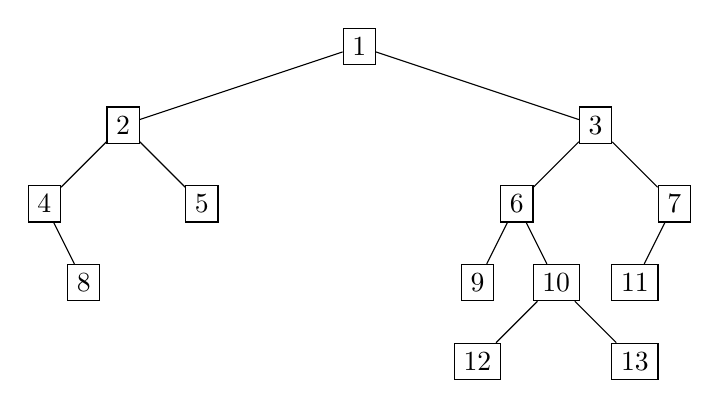
\begin{tikzpicture}
\node[draw] (1) at (0,0) {1};
\node[draw] (2) at (-3,-1) {2};
\node[draw] (3) at (3,-1) {3};
\node[draw] (4) at (-4,-2) {4};
\node[draw] (5) at (-2,-2) {5};
\node[draw] (6) at (2,-2) {6};
\node[draw] (7) at (4,-2) {7};
\node[draw] (8) at (-3.5,-3) {8};
\node[draw] (9) at (1.5,-3) {9};
\node[draw] (10) at (2.5,-3) {10};
\node[draw] (11) at (3.5,-3) {11};
\node[draw] (12) at (1.5,-4) {12};
\node[draw] (13) at (3.5,-4) {13};

\draw (1) -- (2);
\draw (1) -- (3);
\draw (2) -- (4);
\draw (2) -- (5);
\draw (3) -- (6);
\draw (3) -- (7);
\draw (4) -- (8);
\draw (6) -- (9);
\draw (6) -- (10);
\draw (7) -- (11);
\draw (10) -- (12);
\draw (10) -- (13);
\end{tikzpicture}
\captionof{figure}{Arbre binaire}
\label{arbre2}
\end{center}
\begin{enumerate}
\item Effectuer les parcours suivants dans l'arbre figure \ref{arbre2}:
\begin{itemize}
\item en largeur,
\item préfixe,
\item infixe,
\item postfixe.
\end{itemize}
\item Quelle est la hauteur de cet arbre. On considère qu'un arbre vide à une hauteur de -1.
\item Cet arbre est-il équilibré?
\item Cet arbre est-il complet?
\end{enumerate}
\end{exo}
\begin{exo}
En généalogie le principe de la numérotation de Sosa-Stradonitz attribue le numéro 1 à l’individu racine (le sujet sur lequel on établit l’ascendance) puis le numéro 2 à son père et 3 à sa mère. Ainsi, chaque homme a un numéro double de celui de son enfant et donc pair et chaque femme un numéro double de celui de son enfant plus un, soit un numéro impair.
\begin{enumerate}
\item Le numéro 17 est-il une femme ou un homme? Quel est les numéros de son père et sa mère? Quel est le numéro de son enfant?
\item Combien de trisaïeuls (ancêtres de quatrième degré) possède un individu?
\item Un généalogiste propose d'imprimer l'arbre généalogique d'un individu avec quatre degrés d'ascendance. Combien de personnes seront affichées dans cet arbre?
\end{enumerate}
L'arbre des ascendants d'Emmanuel Macron est représenté dans un liste Python (code \ref{manu}).
\begin{center}
\lstinputlisting[firstline=10,lastline=15,xleftmargin=2em, xrightmargin=2em]{"scripts/arbre-genealogique.py"}
\captionof{code}{Représentation en mémoire d'un arbre généalogique}
\label{manu}
\end{center}
\begin{enumerate}[resume]
\item Représenter l'arbre généalogique sous forme d'un arbre binaire.
\item Ouvrir le fichier \emph{arbre-genealogique.py}.
\item Écrire la fonction \textbf{get\_parents(tab: list, id\_enfant: int)$\;\rightarrow\;$tuple} qui renvoie le nom des parents de \emph{id\_enfant} sous forme de tuple. La fonction devra gérer les identifiants trop grands à l'aide d'une assertion.
\item Écrire la fonction \textbf{ascendant\_homme(tab: list, hommes: list)$\;\rightarrow\;$list} qui renvoie la liste des hommes de la personne dont on a réalisé l'arbre généalogique. La fonction devra parcourir l'arbre en profondeur. De plus une simple liste Python fera office de pile.
\item Écrire une version récursive de la fonction précédente.
\end{enumerate}
\end{exo}
nombre de feuilles (récursif)\\
insertion, suppression\\
binarytree\\
tri par tas\\
numérotation de Sosa-Stradonitz
\end{Form}
\end{document}